% ARGUES: the registered E1 and E2 results, reported once, whichever way they land.
% DRAWS FROM: the one-shot confirmatory fit, run 2026-08-31.
%   data/analysis/phase_c/{e1,e2}_{corrected,registered}_nobootstrap.json
%
% FILLED 2026-09-04 from the fit. Every number below is read from those four
% artifacts. Nothing here is provisional in the \prov{} sense: the fit is final
% and the pending bootstrap pass cannot change a coefficient, a p-value or a
% directional decision, only add percentile intervals.
%
% ORDERING NOTE. E1 is reported before E2, which is the pre-registered order,
% even though the paper leads with E2 in the abstract, introduction and
% discussion. Reordering the results table so the supported hypothesis comes
% first is exactly the appearance the reframe must avoid. Frame in the
% discussion; report in registered order here. Do not "fix" this.

\section{Results}
\label{sec:results}

Results are reported under both pipelines that §11 sub-amendment \#12 commits us
to: the corrected pipeline, which applies the re-judgments of the 6,852 at-risk
citations, and the registered pipeline, which applies amendment \#6(c) exactly as
written. The two agree on every directional decision and every significance call
reported in this section. Where they differ in magnitude, both magnitudes are
given and the corrected value is named first.

\subsection{E1: the checkpoint cascade}

The confirmatory model is the parsimony-primary specification of §6,
\texttt{fabricated \textasciitilde{} stage\_ordinal * cell * domain + (1 |
family/model\_id) + (1 | question\_id)}, fitted to 42,845 generations from 12
checkpoints across 900 questions.

\paragraph{The registered interaction did not reject.}
H1.1 predicted a stage-by-cell interaction with the steepest rise in
obscure-but-real. The interaction term
\texttt{stage\_ordinal:cellobscure\_real} is small, positive and not
significant: $\hat\beta = 0.084$ (SE 0.054), $\mathrm{OR} = 1.09$, Wald 95\% CI
$[0.98, 1.21]$, $p = 0.120$, Holm-adjusted $p = 0.360$. Under the registered
pipeline it is smaller still, $\hat\beta = 0.036$ (SE 0.057), $\mathrm{OR} =
1.04$, $[0.93, 1.16]$, $p = 0.531$, Holm-adjusted $p = 1.000$. We report this as
a null result, not as a trend.

\paragraph{The stage main effect is large.}
What the same model does show is a steep, cell-independent rise with
post-training stage: $\hat\beta = 0.881$ (SE 0.174) per stage,
$\mathrm{OR} = 2.41$, $[1.72, 3.39]$, Holm-adjusted $p = 1.5 \times 10^{-6}$
(registered: $0.861$, SE 0.173, $\mathrm{OR} = 2.37$, $[1.69, 3.32]$,
Holm-adjusted $p = 2.6 \times 10^{-6}$). Fabrication does rise sharply with
post-training. It does not rise preferentially in the cell where H1.1 predicted
it would.

\paragraph{The unanswerable interaction is negative.}
\texttt{stage\_ordinal:cellunanswerable} is negative and strongly significant:
$\hat\beta = -0.356$ (SE 0.049), $\mathrm{OR} = 0.70$, $[0.64, 0.77]$,
Holm-adjusted $p = 2.2 \times 10^{-12}$ (registered: $-0.402$, SE 0.052,
$\mathrm{OR} = 0.67$, $[0.60, 0.74]$, Holm-adjusted $p = 3.3 \times 10^{-14}$).
Relative to known-real, fabrication on unanswerable items climbs more slowly
with stage. Section~\ref{sec:discussion} notes that a ceiling reading is
available for this and that the design does not test it.

\paragraph{Neither domain moderator rejected.}
Both third-order terms are indistinguishable from zero:
medical $\hat\beta = -0.019$ (SE 0.076) and legal $\hat\beta = -0.041$
(SE 0.095), Holm-adjusted $p = 1.000$ for both, and likewise under the
registered pipeline ($-0.027$ and $0.002$).

\begin{table}[t]
\centering
\small
\caption{T4. The registered E1 family of five, Holm-corrected within the family.
Corrected pipeline first, registered pipeline in parentheses. Odds ratios are
per unit of \texttt{stage\_ordinal}; intervals are Wald.}
\label{tab:t4}
\begin{tabular}{lrrrl}
\toprule
Term & $\hat\beta$ & OR & Wald 95\% CI & Holm $p$ \\
\midrule
\texttt{stage\_ordinal}
  & 0.881 & 2.41 & [1.72, 3.39] & $1.5\times10^{-6}$ \\
  & (0.861) & (2.37) & ([1.69, 3.32]) & ($2.6\times10^{-6}$) \\
\texttt{stage\_ordinal:cellobscure\_real}
  & 0.084 & 1.09 & [0.98, 1.21] & 0.360 \\
  & (0.036) & (1.04) & ([0.93, 1.16]) & (1.000) \\
\texttt{stage\_ordinal:cellunanswerable}
  & $-0.356$ & 0.70 & [0.64, 0.77] & $2.2\times10^{-12}$ \\
  & ($-0.402$) & (0.67) & ([0.60, 0.74]) & ($3.3\times10^{-14}$) \\
\texttt{...:cellobscure\_real:domainmedical}
  & $-0.019$ & 0.98 & [0.85, 1.14] & 1.000 \\
  & ($-0.027$) & (0.97) & ([0.83, 1.14]) & (1.000) \\
\texttt{...:cellobscure\_real:domainlegal}
  & $-0.041$ & 0.96 & [0.80, 1.16] & 1.000 \\
  & (0.002) & (1.00) & ([0.83, 1.21]) & (1.000) \\
\bottomrule
\end{tabular}
\end{table}

\paragraph{The directional check passed; the co-primary rule did not.}
Within obscure-but-real, the marginal fabrication probability rises from 4.78\%
at base to 56.66\% at RLHF, an increase of 51.9 percentage points, which clears
the pre-committed 10-point threshold (registered: 4.46\% to 49.77\%, 45.3
points, also clearing it). The co-primary rule of §6 sensitivity \#5 is an
intersection-union: the headline T1 claim holds only if both the continuous
interaction and the binary base-versus-post contrast reject. The binary contrast
does not ($p = 0.588$; registered $p = 0.514$), and neither does the continuous
interaction, so \textbf{the headline T1 claim is not supported} under either
pipeline.

The two components of that rule failed in different ways, and the distinction
matters for the title. The pre-registration ties the null title
\emph{Citation Fabrication Does Not Cleanly Track Post-Training Stage} to a
failure of the \emph{directional} check, and the directional check passed.
What failed is the interaction test. The honest summary is that fabrication
tracks post-training stage steeply but does not track it differentially by cell.

We therefore do not use the null title. Its registered trigger, a failed
directional check, did not occur on either roster, and swapping titles on a
different failure than the one registered would be an outcome-driven change of
its own. The title the paper carries makes no claim about T1 in either
direction: it names the two manipulations studied, and the abstract states that
the T1 interaction was not supported.

\begin{figure}[t]
\centering
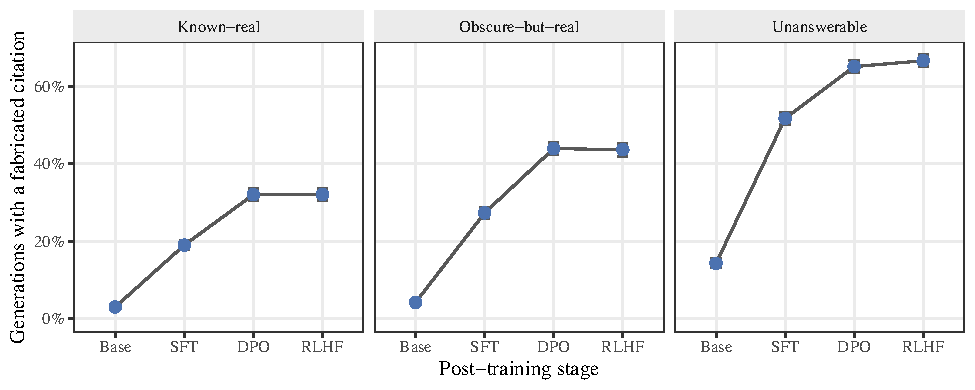
\includegraphics[width=\textwidth]{f1_stage_by_cell}
\caption{Observed fabrication rate by post-training stage, within each question
cell. Points are raw proportions of generations carrying at least one fabricated
citation, with 95\% Wilson intervals. They are not the marginal probabilities
quoted in the text, which come from the fitted model and weight cells equally;
the figure shows shape and the tables carry the inference. Two things are
visible at once. Fabrication rises steeply from base to SFT in all three cells
and then flattens, and the three cells rise more or less together. That
combination, a large stage main effect with no differential slope by cell, is
exactly what leaves the registered T1 interaction null. $n = 42{,}845$
generations over 12 checkpoints.}
\label{fig:f1}
\end{figure}

\subsection{E2: prompt-condition manipulation}

The confirmatory model is \texttt{fabricated \textasciitilde{} condition *
is\_post\_trained * cell + domain + (1 | family/model\_id) + (1 |
question\_id)}, fitted to the same 42,845 generations. All 12 checkpoints in the
frozen set are open-weights, so the primary open-weights subsample is the whole
frame.

\paragraph{H1.2 is strongly supported.}
The condition-by-post-trained interaction is the largest effect in the study:
$\hat\beta = 4.62$ (SE 0.374), $z = 12.37$, $\mathrm{OR} = 101.6$, Wald 95\% CI
$[48.8, 211.3]$, Holm-adjusted $p = 2.0 \times 10^{-34}$. The registered
pipeline reproduces it at a smaller magnitude, $\hat\beta = 4.02$ (SE 0.416),
$z = 9.67$, $\mathrm{OR} = 55.5$, $[24.6, 125.4]$, Holm-adjusted
$p = 2.1 \times 10^{-21}$. The gap runs in the direction sub-amendment \#12
predicts, since the withheld correction suppresses measured fabrication most in
\texttt{citations\_expected}, and the registered pipeline is therefore the
conservative one on this contrast as well.

Moving to the maximal random-effects structure raises the estimate rather than
shrinking it, $\hat\beta = 5.61$ (SE 0.750), $z = 7.48$, $\mathrm{OR} = 273.9$,
$[62.9, 1191.8]$, $p = 3.7 \times 10^{-13}$ on the corrected pipeline, so the
interaction is not an artifact of the parsimony-primary random-effects choice.
That fit is singular, and Appendix~\ref{app:supplementary} reports both the full
coefficient tables and the rePCA locating the singularity in the three-level
family factor.

\paragraph{The cue moves base and post-trained checkpoints in opposite directions.}
This is the result the paper leads with, and it is worth stating on the
probability scale. Asking for citations \emph{lowers} fabrication in base
checkpoints, from 9.04\% under the neutral prompt to 0.77\%, a fall of 8.3
points. In post-trained checkpoints the same cue \emph{raises} it, from 34.18\%
to 73.70\%, a rise of 39.5 points. The interaction delta is 47.8 percentage
points, far clear of the pre-committed 10-point threshold. The registered
pipeline reproduces the sign reversal at a smaller magnitude: 8.68\% to 0.72\%
for base, 31.73\% to 57.22\% for post-trained, an interaction delta of 33.5
points.

The reversal holds in every domain, and it is not an artifact of one of them:
the interaction delta is 48.5 points in academic, 48.9 in medical and 42.5 in
legal, all three clearing the threshold (registered: 34.3, 36.1 and 29.3).

\begin{table}[t]
\centering
\small
\caption{T5. E2 marginal fabrication probabilities by prompt condition and
post-training status, corrected pipeline with registered pipeline in
parentheses. The interaction delta is the post-trained rise minus the base
rise.}
\label{tab:t5}
\begin{tabular}{lrrr}
\toprule
 & Neutral & Citations expected & Difference \\
\midrule
Base checkpoints        & 9.04\% (8.68\%)  & 0.77\% (0.72\%)   & $-8.3$ ($-8.0$) pts \\
Post-trained checkpoints & 34.18\% (31.73\%) & 73.70\% (57.22\%) & $+39.5$ ($+25.5$) pts \\
\midrule
Interaction delta       &                  &                   & \textbf{47.8 (33.5) pts} \\
\bottomrule
\end{tabular}
\end{table}

\paragraph{The closed-API secondary block is empty.}
H1.2b was registered against a closed-API subsample. The frozen checkpoint set
contains no closed-API models, so the secondary block carries no formula, no
coefficients and no directional result. H1.2b is untested rather than
unsupported, and no claim about closed or frontier models follows from this
study.

\subsection{The de-confounding contrast: the citation cue, not the length demand}

The \texttt{length\_matched} condition exists to separate ``asked for citations''
from ``asked for a longer answer.'' Amendment \#10 pins the quantity that decides
it: $\Delta$ is the \texttt{emmeans} marginal probability-scale contrast
\texttt{citations\_expected} minus \texttt{length\_matched}, proportional weights
over cells and domains, evaluated at the \texttt{is\_post\_trained}~$=1$ margin of
the same GLMM that yields the registered E2 test. The bin boundaries at
$\pm 5$pp, and the rule that a point estimate within 2pp of a boundary whose CI
crosses it is reported as boundary-ambiguous, were fixed before any Phase C
number bearing on this contrast existed.

\begin{table}[htbp]
\centering
\small
\caption{Amendment \#10 de-confounding contrast, both pipelines. Probabilities
are marginal at \texttt{is\_post\_trained}~$=1$. The registered pipeline is the
one that withholds the verifier-REAL correction of amendment \#12.}
\label{tab:amd10}
\begin{tabular}{@{}l r r@{}}
\toprule
 & Corrected & Registered \\
\midrule
$P(\text{fab} \mid \texttt{citations\_expected})$ & 0.7380 & 0.5728 \\
$P(\text{fab} \mid \texttt{length\_matched})$     & 0.4545 & 0.4465 \\
$P(\text{fab} \mid \texttt{neutral})$             & 0.3428 & 0.3177 \\
\midrule
$\Delta$ (percentage points) & $+28.35$ & $+12.64$ \\
95\% CI                      & $[+25.58, +31.12]$ & $[+10.75, +14.53]$ \\
\textbf{Registered bin}      & \textbf{citation cue supported} & \textbf{citation cue supported} \\
\midrule
Secondary, all open-weights  & $+20.89$ & $+9.06$ \\
95\% CI                      & $[+18.80, +22.98]$ & $[+7.61, +10.50]$ \\
\midrule
OR \texttt{citations\_expected} vs neutral & 5.40 & 2.88 \\
OR \texttt{length\_matched} vs neutral     & 1.60 & 1.73 \\
\bottomrule
\end{tabular}
\end{table}

$\Delta$ lands in the $\Delta \geq +5$pp bin under both pipelines, and not
marginally: the lower confidence bound is $+25.58$pp corrected and $+10.75$pp
registered, so neither interval comes near the boundary and the boundary rule
does not engage. \textbf{The citation cue, not the verbosity demand, drives the
effect}, and T2's citation-specific reading is supported by this contrast. The
odds-ratio ordering agrees in both pipelines, with
\texttt{citations\_expected} above \texttt{length\_matched} rather than below it.

Three things about this result deserve stating plainly rather than being left for
a reader to reconstruct.

First, \textbf{it reverses the direction the amendment was written to
accommodate}. The exploratory Phase B prior, on a single closed-API model, put
$\Delta$ at roughly $-2$pp on this scale with \texttt{length\_matched} above
\texttt{citations\_expected}, and amendment \#10 exists because that ordering
made a registered loss for T2 look plausible. It did not transfer. The amendment
anticipated exactly this, warning that a single small closed-API model's
length-compliance behavior may not carry to open-weights checkpoints with
different post-training pipelines, and that the Phase C result is the primary
evidence. The elaborate negative-delta machinery was built for a case that did
not occur, and it is reported here as a rule that was fixed in advance and did
not fire, not as a rule that was never needed.

Second, \textbf{the two pipelines agree on the bin while differing substantially
in magnitude}, $+28.35$pp against $+12.64$pp. That gap is in the direction
sub-amendment \#12 predicted and for the reason it gave: the verifier-REAL trust
failure suppresses measured fabrication differentially, and its exposure is
highest in \texttt{citations\_expected} (26.4\% of generations at risk, mean 1.64
trusted citations) and lowest in \texttt{length\_matched} (14.6\%, 1.09). The
uncorrected pipeline therefore understates precisely this contrast. What matters
for the registered conclusion is that the \emph{more conservative} pipeline still
clears the boundary by a wide margin, so the finding does not depend on the
correction.

Third, the marginal probabilities here differ in the third significant figure
from those in Table~\ref{tab:t5} (0.3428 against 34.18\%, 0.7380 against
73.70\%). That is not an inconsistency: amendment \#10 specifies proportional
weights over cells and domains, whereas the directional check of §6 uses
\texttt{emmeans}'s equal weighting. The two answer slightly different questions
and the registered one is used for the bin.

\begin{figure}[t]
\centering
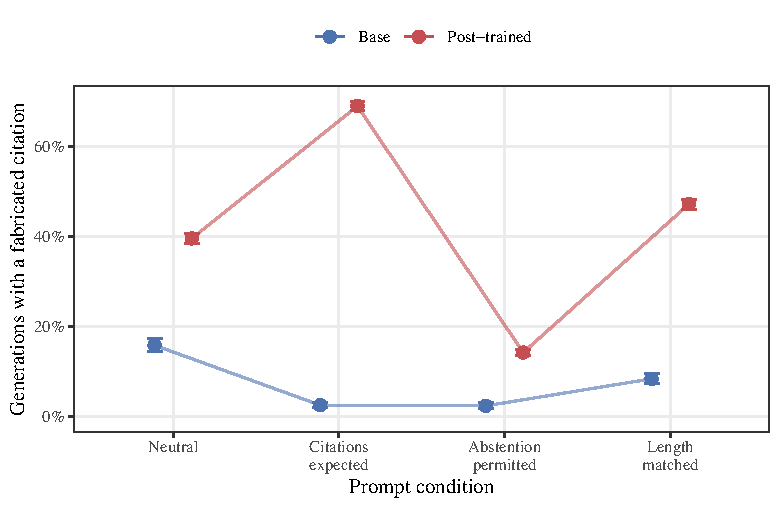
\includegraphics[width=0.74\textwidth]{f2_condition_by_stage}
\caption{Observed fabrication rate by prompt condition, split by whether the
checkpoint has been post-trained, with 95\% Wilson intervals. This is the
interaction that H1.2 predicted, and it is visible without a model: asking for
citations moves the two groups in \emph{opposite} directions. Base checkpoints
fall from 15.8\% under the neutral prompt to 2.5\% when citations are requested,
while post-trained checkpoints rise from 39.5\% to 68.9\%. The length-matched
control, which demands a longer answer without mentioning citations, lands well
below the citation cue for post-trained checkpoints (47.1\% against 68.9\%),
which is the de-confounding contrast of amendment \#10 in raw form. Base rates
are computed on 2,686 to 2,700 generations per condition and post-trained rates
on 7,985 to 8,047.}
\label{fig:f2}
\end{figure}

\subsection{Sensitivity analyses}

\paragraph{Stage as a four-level factor.}
Treating stage as a factor rather than a linear score shows where the rise
happens. Against base, the odds ratios are 10.04 $[5.46, 18.43]$ for SFT,
17.10 $[9.32, 31.35]$ for DPO and 17.01 $[9.28, 31.19]$ for RLHF. Most of the
movement is already present at SFT, and DPO and RLHF are indistinguishable from
each other. The cascade is not a story about the final preference-optimization
step.

\paragraph{Verbosity does not explain the null.}
The registered covariate-adjusted model adds citation count as a verbosity
proxy. Verbosity is itself a powerful predictor, $\hat\beta = 1.468$ (SE 0.040),
$\mathrm{OR} = 4.34$, $[4.01, 4.70]$. The primary interaction remains null with
it in the model, $\hat\beta = 0.032$ (SE 0.055), $p = 0.561$. The H1.1 null is
not a verbosity artifact in either direction.

\paragraph{The extended random-effects fit is singular.}
The maximal random-effects specification converged but is singular in both E1
and E2, so the operative-model rule of §6 selects the parsimony-primary fit,
which is the model reported throughout this section.

\paragraph{The MISGROUNDED category is empty.}
Section 6 commits to reporting FABRICATED and MISGROUNDED separately rather than
only summed, on the grounds that MISGROUNDED (a real work, a wrong claim) is the
cleaner reward-hacking signal because it controls for retrieval capability. In
the judged data the MISGROUNDED rate is zero, so the combined rate equals the
fabricated rate: 33.56\% under the corrected pipeline and 30.16\% under the
registered one, against an abstention rate of 41.24\% and a mean of 0.944 cited
works per generation. The registered split therefore cannot be reported as
intended, and the reason belongs in Section~\ref{sec:instrument} rather than
here.

\paragraph{Recoding unverifiable citations as fabricated.}
The primary analysis excludes a generation that cited only unverifiable sources,
because it carries neither a good nor a bad citation. That exclusion conditions
on ``the model cited something verifiable,'' which is post-treatment if
unverifiable rates differ by stage. Sensitivity \#1 recodes those citations as
fabricated instead, and its virtue is that it \textbf{excludes nothing by
construction}: the analysis frame goes from 42{,}845 generations to all 43{,}200,
so the missingness question is dissolved rather than argued.

The registered escalation trigger asked whether the exclusion rate is monotone in
stage within the obscure-but-real cell. Pooled, it is not: 2.25\%, 2.85\%,
2.58\%, 2.21\% across the four stages, so the literal trigger returns false. We
ran the sensitivity as co-primary anyway, a deviation recorded before the
confirmatory fit and explained in Appendix~\ref{app:deviations}. The reason is
that the pooled test masks the legal domain, which \emph{is} monotone decreasing
across all four stages (7.84\%, 7.72\%, 6.24\%, 5.55\%) at roughly thirty times
the academic rate, and which the pooled $n$ drowns out. Running a sensitivity
that turns out to be unnecessary costs a paragraph; omitting one that turns out
to be necessary is not recoverable after a one-shot fit.

It changes nothing. Under both pipelines the recoded analysis returns
\texttt{headline\_t1\_supported} false, for the same reasons and with
substantially the same coefficients. The registered interaction remains null
($\hat\beta = 0.085$, Holm $p = 0.349$ corrected; $\hat\beta = 0.037$, Holm
$p = 1.000$ registered), the co-primary binary contrast does not reject
($p = 0.580$ and $p = 0.508$), the stage main effect remains large
($\mathrm{OR} = 2.41$ and $2.37$ per stage), and the stage-by-unanswerable
interaction remains negative and significant. The directional check passes in
both, rising 5.80\% to 59.42\% corrected and 5.45\% to 52.94\% registered. The
E1 conclusion is therefore robust to the one analytic choice that could have
manufactured it through informative exclusion.

The same re-coding on E2 moves the headline result slightly \emph{away} from the
null under both pipelines. On the 43,200-generation frame the
condition-by-post-trained interaction is $\hat\beta = 4.77$ (SE 0.370),
$\mathrm{OR} = 118.5$ $[57.3, 244.8]$, Holm-adjusted
$p = 2.4 \times 10^{-37}$ corrected, against $\hat\beta = 4.22$ (SE 0.412),
$\mathrm{OR} = 68.2$ $[30.4, 152.8]$, $p = 5.6 \times 10^{-24}$ registered. Both
are larger than their primary counterparts of 4.62 and 4.02. The directional
check passes in both, at 48.4 and 35.1 points, and the amendment \#10 contrast
stays in the citation-cue bin under both, at $+25.86$pp and $+11.41$pp. Treating
every unresolvable citation as a fabrication does not weaken H1.2, which is what
one would expect if the effect were being carried by differential missingness
rather than by the cue.

\subsection{The fifteen-model refit}
\label{sec:refit15}

Amendment \#13 (Appendix~\ref{app:deviations}) records that the twelve
checkpoints above are 12 of the 23 registered, and that three more registered
checkpoints were collected under a rule fixed before any of their generations
existed: Llama-3.1-70B-Instruct, which joins the Tülu-3-70B family as a second
post-trained branch off the same base, and the Qwen2.5-72B base and Instruct
pair as a fourth family. The refit uses the same registered specification, both
pipelines and Wald intervals (amendment \#14), on 53,620 generations from 15
checkpoints. A-priori power on this roster is 83.0\% for the E1 interaction and
83.5\% for the E2 interaction at nominal $\alpha$, against 73.0\% for both on
the twelve; neither clears the 80\% gate at the Holm floor. The twelve-model fit
remains the registered one-shot result on the roster that ran. The refit is
reported beside it, not in place of it, and nothing in it was used to decide
what to collect.

\paragraph{E1: the registered interaction is still null, and T1 is still not supported.}
\texttt{stage\_ordinal:cellobscure\_real} is now slightly \emph{negative}:
$\hat\beta = -0.071$ (SE 0.042), $\mathrm{OR} = 0.93$ $[0.86, 1.01]$,
$p = 0.096$, Holm-adjusted $p = 0.192$ (registered: $-0.070$, $\mathrm{OR} =
0.93$ $[0.85, 1.02]$, Holm-adjusted $p = 0.250$). With power above the gate, this
null is more informative than the twelve-model one, and its point estimate
points away from the registered prediction rather than toward it. The stage
main effect remains large, $\mathrm{OR} = 1.92$ $[1.33, 2.78]$ per stage,
Holm-adjusted $p = 0.0020$ (registered 1.89, $p = 0.0022$), and the
unanswerable interaction remains negative, $\mathrm{OR} = 0.68$ $[0.63, 0.74]$,
Holm-adjusted $p = 2.6 \times 10^{-20}$. Neither domain moderator survives Holm
(legal $\mathrm{OR} = 1.15$, unadjusted $p = 0.045$, Holm $0.136$; medical
$1.09$, Holm $0.192$). Within obscure-but-real the marginal probability rises
from 8.10\% at base to 44.76\% at the final stage, 36.7 points (registered
7.28\% to 38.53\%, 31.2 points), so the directional check passes again.

One component of the co-primary rule changes. The binary base-versus-post
contrast, which did not reject on twelve checkpoints, rejects on fifteen
($p = 4.7 \times 10^{-5}$ corrected, $p = 0.0039$ registered). The rule is an
intersection-union and the continuous interaction still does not reject, so
\textbf{\texttt{headline\_t1\_supported} remains false under both pipelines}. The
stage-as-factor sensitivity explains why the two components now disagree: every
stage-by-obscure-real term is \emph{below} one (SFT 0.47, DPO 0.62, final 0.56,
all $p < 0.004$ corrected), so on fifteen checkpoints obscure-but-real
fabrication rises \emph{less} steeply than known-real, the reverse of H1.1.

\paragraph{E2: the interaction holds, at a smaller magnitude.}
The condition-by-post-trained interaction is again the strongest registered
effect: $\hat\beta = 1.91$ (SE 0.162), $z = 11.76$, $\mathrm{OR} = 6.75$
$[4.91, 9.29]$, Holm-adjusted $p = 3.2 \times 10^{-31}$ (registered:
$\hat\beta = 1.38$, $\mathrm{OR} = 3.98$ $[2.83, 5.61]$, Holm-adjusted
$p = 1.3 \times 10^{-14}$). On the probability scale the post-trained rise is
almost unchanged, 35.16\% to 74.91\%, 39.8 points, and the interaction delta is
41.5 points (registered 32.09\% to 58.55\%, 26.5 points; delta 28.9). It
clears the 10-point threshold in every domain: 41.4 academic, 38.4 medical,
40.5 legal (registered 28.7, 29.8, 27.3).

\paragraph{What changes is the base side.}
On twelve checkpoints the citation cue pushed base checkpoints down by 8.3
points. On fifteen the base marginal barely moves, 11.87\% to 10.08\%, a fall of
1.8 points (registered 2.4), and the conditional base-model odds ratio for
\texttt{citations\_expected} turns above one ($\mathrm{OR} = 1.54$
$[1.15, 2.07]$, Holm-adjusted $p = 0.0071$; registered 1.43, Holm-adjusted
$p = 0.057$). The change comes from one checkpoint. Raw rates for the four base
checkpoints, neutral against citations-expected, are 7.4\% to 0.0\% for
OLMo-2-13B, 17.0\% to 7.2\% for Llama-3.1-8B, 23.0\% to 0.2\% for
Llama-3.1-70B, and \textbf{47.8\% to 71.7\% for Qwen2.5-72B}, which responds to
the cue the way the post-trained checkpoints do. We do not know why. The
checkpoint is labeled a base model by its release, and the label is what the
design codes, so the result is reported as observed. What survives both rosters
is the interaction and the post-trained rise. The claim that the cue moves base
checkpoints \emph{down} holds for the three base models in the original roster
and not for the fourth, and the paper does not make it as a general statement.

\paragraph{Sensitivities on fifteen checkpoints.}
The maximal random-effects fit is singular again in both experiments, so the
parsimony-primary fit stays operative; its E2 interaction is larger, not
smaller ($\mathrm{OR} = 106.4$ corrected, 32.0 registered). Adding citation
count as a verbosity covariate shrinks the E2 interaction substantially, to
$\mathrm{OR} = 2.28$ $[1.63, 3.20]$, $p = 1.8 \times 10^{-6}$ corrected and
1.48 $[1.03, 2.12]$, $p = 0.032$ registered (on twelve: 9.46 and 4.88). Part of
the cue effect therefore runs through the cue making post-trained checkpoints
cite more, which is the same pattern E4 found for the naive judge. The
de-confounding contrast of amendment \#10 on fifteen checkpoints lands in the
same bin as on twelve: $\Delta = +28.10$pp $[+23.35, +32.85]$ corrected and
$+13.19$pp $[+11.46, +14.91]$ registered, both ``citation cue supported'' and
both clear of the $\pm 5$pp boundary (twelve-model values $+28.35$ and
$+12.64$). Sensitivity \#1, which recodes unverifiable citations as fabricated
and so excludes nothing (54,000 generations), changes no conclusion: the E1
interaction stays null (Holm-adjusted $p = 0.188$ corrected, $0.235$
registered), the binary contrast still rejects, \texttt{headline\_t1\_supported}
stays false, and the E2 interaction strengthens slightly ($\mathrm{OR} = 7.51$,
Holm-adjusted $p = 2.1 \times 10^{-36}$ corrected; 4.54,
$2.0 \times 10^{-18}$ registered). The selection check's registered trigger does not
fire on fifteen checkpoints either (pooled obscure-real exclusion 1.27\%,
2.85\%, 2.58\%, 1.60\% by stage). The drift diagnostics D1 to D3 are identical
to the twelve-model values, as they must be: the three new checkpoints were
judged in a single later run with healthy grounding and carry no judge era, so
they drop out of those models.

\paragraph{The amendment \#14 escalation check.}
Amendment \#14 keeps the profile-likelihood escalation and applies it to the
Wald lower bound of each directional contrast on the probability scale. On both
rosters and both pipelines, no domain-marginal contrast comes near the 12-point
trigger: the lowest lower bound is 14.0 points (E1, fifteen checkpoints,
registered pipeline; 18.1 corrected), and no E2 lower bound, marginal or per
domain, falls below 22.6 points. So the rule does not fire on any registered estimand. Two of the
per-domain breakdowns, which are reported for heterogeneity and are not the
registered estimand, do come close on the fifteen-model registered pipeline:
the E1 rise in academic has a lower bound of 9.1 points and in legal 11.1. We
report them rather than escalate them, and note that the corrected pipeline
puts both only just above the trigger (12.1 and 12.04 points).

\guide{The era-stratified robustness panel belongs in
Section~\ref{sec:instrument}, not here, because it re-estimates registered
contrasts and is gated behind an explicit flag for that reason.}
